\subsection{Decorator (\textit{o Wrapper})}
\label{decorator}

\textbf{Scopo}: Strutturale \\
\textbf{Raggio d'azione}: Oggetti

\paragraph{Definizione} Il pattern decorator permetter di aggiungere dinamicamente responsabilità ad un oggetto. Fornisce un'alternativa flessibile all'uso dell'ereditarietà come strumento per l'estensione delle funzionalità.

\paragraph{Moticazione} Talvolta è necessario aggiungere responsabilità ad un singolo oggetto e non ad un intera classe. Si consideri una libreria per la realizzazione di interfacce utente che deve permettere di aggiungere bordi o altri elementi a ciascun componente grafico. Ricorrere all'ereditarietà complicherebbe la cosa, andrebbero create sottoclassi per ogni componente aggiuntivo, in più renderebbe difficile comporre più estensioni di comportamento.

\begin{figure}[H]
    \centering
    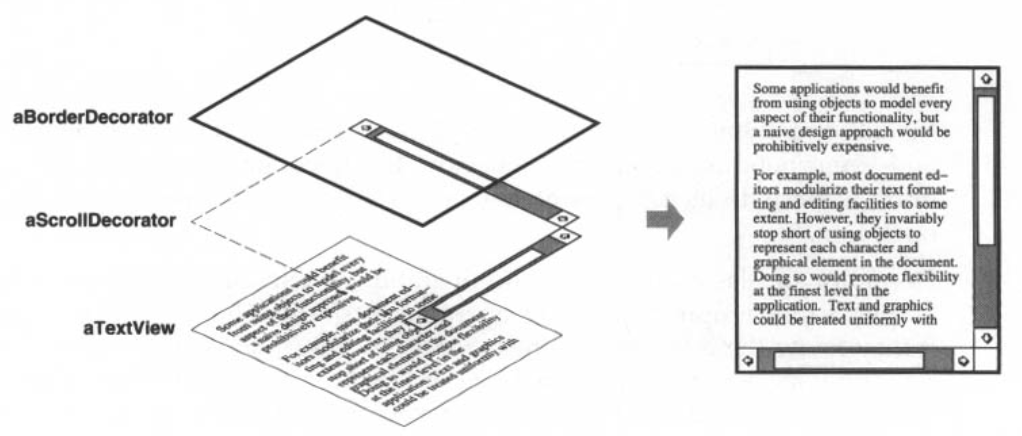
\includegraphics[width=0.5\linewidth]{assets/pattern/decorator/decorator-esempio-grafico.png}
\end{figure}

La soluzione consiste nel racchiudere il componente da decorare dentro un altro che sarà responsabile di disegnare il bordo o aggiungere altri componenti visivi. L'oggetto contenitore è detto \textit{decoratore} ed ha la stessa interfaccia dell'oggetto decorato così da poter essere trasparente al client. È possibile che svolga azioni aggiuntive prima o dopo aver trasferito la richiesta all'oggetto decorato.

\begin{figure}[H]
    \centering
    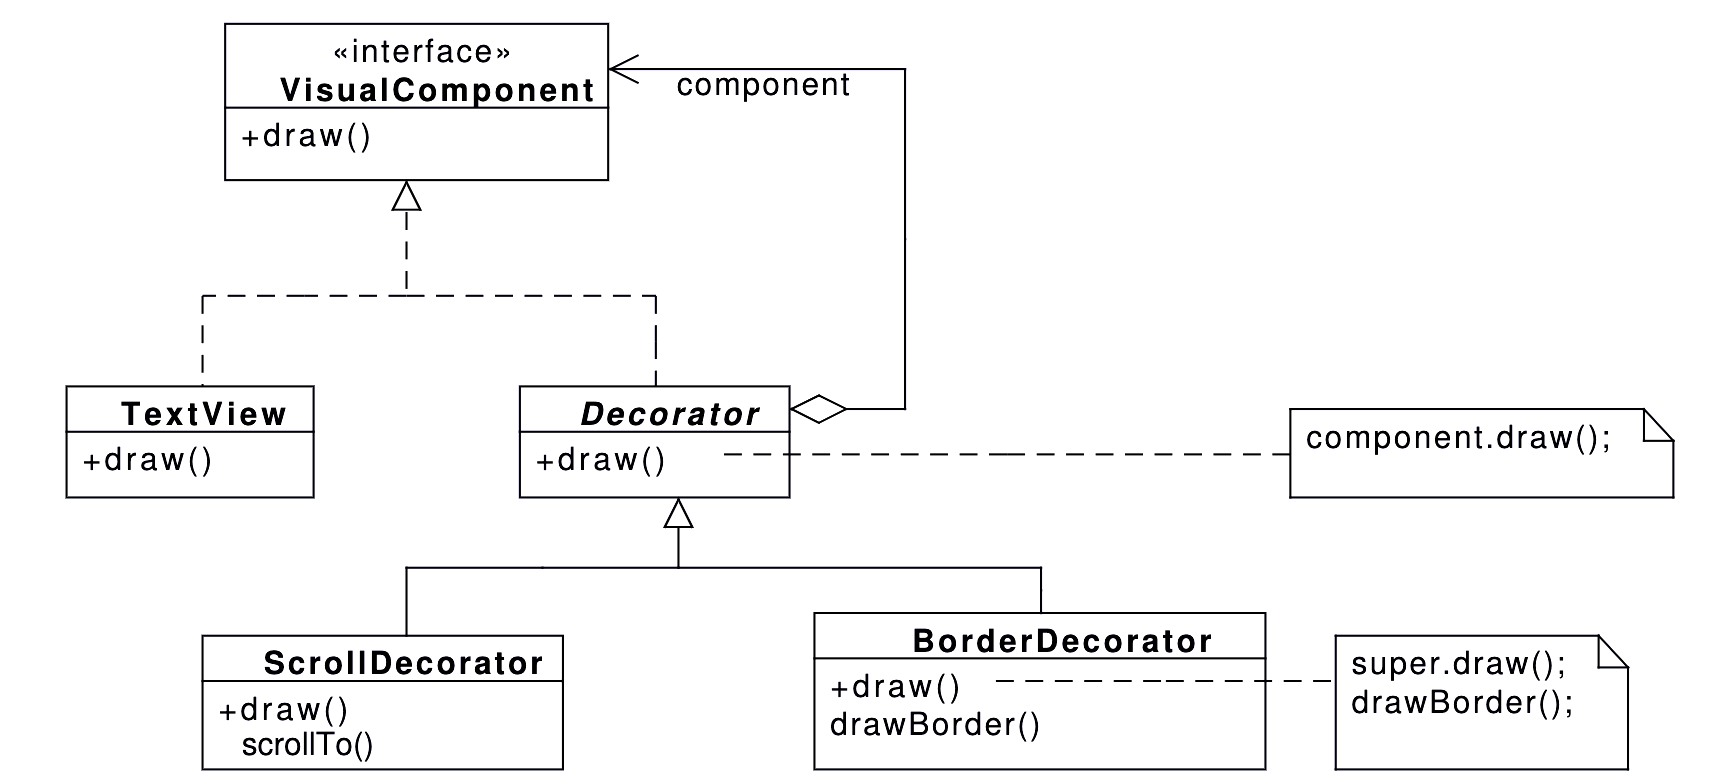
\includegraphics[width=0.75\linewidth]{assets/pattern/decorator/decorator-esempio.png}
    \caption{Esempio di utilizzo del pattern Decorator}
\end{figure}

Nell'esempio l'interfaccia VisualComponent definisce il tipo generico di componenti visuali. La classe TextView consente di visualizzare del testo in una finestra. La classe astratta Decorator inoltra semplicemente le richieste al componente incapsulato. BorderDecorator e ScrollDecorator consentono rispettivamente di aggiungere bordi e barre di scorrimento.

\paragraph{Applicabilità} È consigliabile utilizzare il pattern Decorator quando:
\begin{itemize}
    \item Si vogliono aggiungere responsabilità ad un oggetto dinamicamente e in modo trasparente, senza influenzare altri oggetti;
    \item Si vuole supportare un largo numero di estensioni senza riccorrere all'ereditarietà (che farebbe esplodere il numero di sottoclassi);
\end{itemize}

\begin{figure}[H]
    \centering
    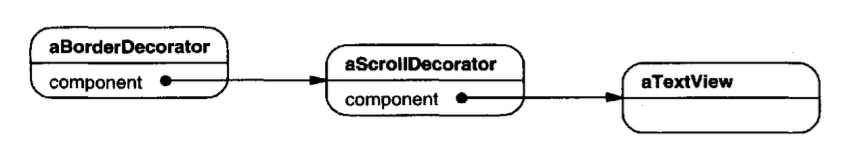
\includegraphics[width=0.75\linewidth]{assets/pattern/decorator/decorator-object-diagram.png}
    \caption{Object Diagram del pattern Decorator}
\end{figure}

\paragraph{Struttura} Il pattern è composto dai seguenti partecipanti:
\begin{itemize}
    \item \textbf{ServiceIF} (VisualComponent): definisce l'interfaccia comune per gli oggetti ai quali possono essere aggiunte nuove responsabilità dinamicamente.
    \item \textbf{ConcreteService} (TextView): definisce un oggetto al quale possono essere aggiunte ulteriori responsabilità
    \item \textbf{Decorator}: mantiene un riferimento ad un oggetto di tipo ServiceIF e, al contempo implementa l'interfaccia ServiceIF.
    \item \textbf{ConcreteDecorator} (ScrollDecorator, BorderDecorator): aggiunge responsabilità al componente
\end{itemize}

\begin{figure}[H]
    \centering
    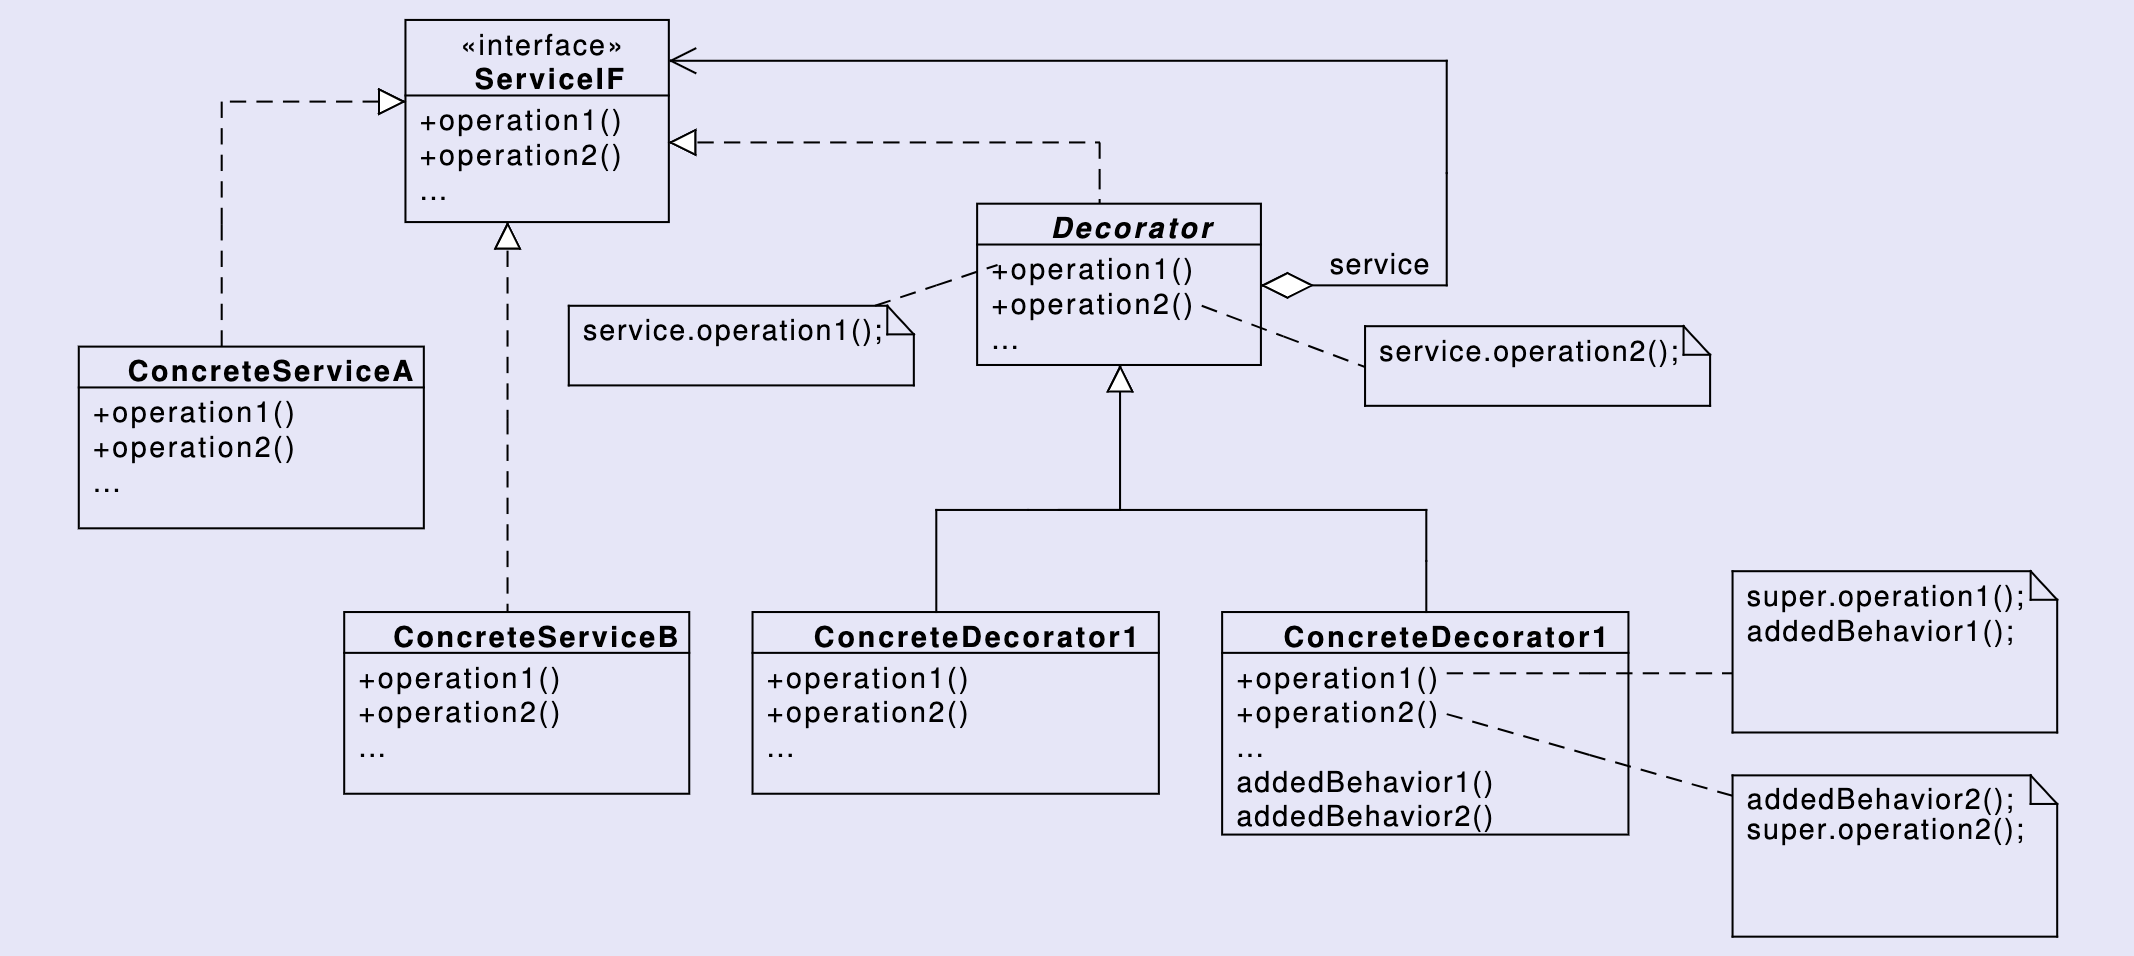
\includegraphics[width=0.75\linewidth]{assets/pattern/decorator/decorator-struttura.png}
    \caption{Class Diagram del pattern Decorator}
\end{figure}

\paragraph{Conseguenze} Il pattern Decorator consente quindi di:
\begin{itemize}
    \item Avere maggiore flessibilità rispetto all'ereditarietà;
    \item Poter utilizzare differenti combinazioni di oggetti attraverso l'utilizzo di diversi decoratori;
\end{itemize}
Inoltre:
\begin{itemize}
    \item L'uso nei progetti porta a sistemi composti di molti oggetti simili interconnessi, facile da interpretare dal progettista, meno da esterni;
    \item Decoratore e oggetto decorato sono uguali in termini di comportamento ma differiscono in termini di identità
    \item Bisogna porre attenzione in come si compongono i decoratori, per esempio evitare dipendenze circolari.
\end{itemize}

\begin{figure}[H]
    \centering
    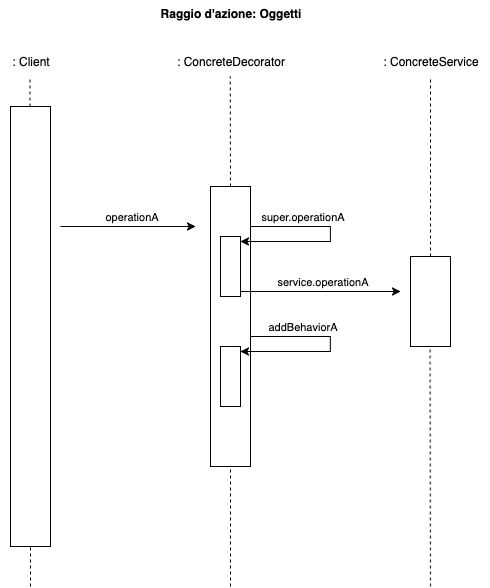
\includegraphics[width=0.75\linewidth]{assets/pattern/decorator/decorator-sequence.drawio.png}
    \caption{Sequence Diagram del pattern Decorator}
\end{figure}


\newpage